\documentclass[conference]{IEEEtran}

% --- IDIOMA ---
\usepackage[spanish, es-tabla]{babel}

% --- FUENTES (XeLaTeX) ---
\usepackage{fontspec}
\setmainfont{Liberation Serif}
\setmonofont{JetBrainsMono Nerd Font}

% --- CITAS IEEE ---
\usepackage[backend=biber,style=ieee,sorting=none]{biblatex}
\addbibresource{referencias.bib}

% --- UTILIDADES ---
\usepackage{graphicx}
\usepackage{float}
\usepackage{amsmath}
\usepackage{booktabs}
\usepackage[colorlinks=true,linkcolor=black,citecolor=black,urlcolor=blue]{hyperref}

% --- CÓDIGO ---
\usepackage{xcolor}
\definecolor{bg}{RGB}{40,44,52}

\usepackage{minted}

\setminted{
  style=monokai,
  bgcolor=bg,
  breaklines,
  breakanywhere=true,
  tabsize=2,
  fontsize=\footnotesize
}

\usepackage{csquotes}

\begin{document}



% --- INICIO DE LA PORTADA ---
\begin{titlepage}
    \centering
    \vspace*{0.5cm}
    
    % --- Escudo de la UV ---
    % Asegúrese de tener el archivo escudo_uv.png (o .jpg) en su carpeta del proyecto
    
\includegraphics[width=0.3\textwidth]{UV.png} \\ 
    \vspace{0.8cm}
    
    {\huge \textbf{Universidad Veracruzana}} \\
    \vspace{0.4cm}
    {\Large Facultad de Instrumentación Electrónica} \\ % Corregido: Instrumentación
    \vspace{0.2cm}
    {\large Ingeniería Biomédica} \\
    
    \vfill
    
    % Título de la Experiencia Educativa y Actividad
    {\Large \textbf{EE: Interfaces Hombre-Máquina}} \\
    \vspace{0.8cm}
    {\Large \textbf{ACTIVIDAD 05. SENSOR PAJ7620 COMO DISPOSITIVO PARA UNA INTERFAZ HOMBRE-MAQUINA SIN CONTACTO}} \\
    
    \vspace{1.5cm}
 
    % Información de los Integrantes
    \begin{flushright} % Alineado a la derecha para un toque más profesional
        \textbf{Profesor:} \\
        Varela Lara Luis Julian \\
        \vspace{0.5cm}
        \textbf{Integrantes del equipo ``\textit{ES3.14}}'': \\
        Alfonso Gamboa Rubén \\
        Flores Montero Edsel Yetlanezi \\
    \end{flushright}
    
    \vfill
    
    {\large \textbf{Fecha:} 20 de mayo de 2026} \\
    \vspace{1cm}
    {\small Xalapa, Enríquez, Ver.} % O la sede correspondiente
\end{titlepage}
% --- FIN DE LA PORTADA ---



% --- EL CUERPO DEL TEXTO (Automáticamente en dos columnas) ---

\section{Introducción al tema.}

El objetivo principal es establecer un sistema físico que permita interactuar en tiempo real con el programa “ComandosRS232”, traduciendo movimientos direccionales de la mano en comandos de navegación para una interfaz gráfica.

A diferencia de los proyectos previos, este diseño aprovecha el reconocimiento óptico de gestos para ejecutar acciones direccionales (arriba, abajo, izquierda, derecha) de forma continua, así como una acción de selección o detención mediante el gesto de ``acercar'' simulando el click de un cursor. Otros temas mencionados anteriormente, serán omitidos para evitar redundancia.

 \subsection{Marco teórico}
  \subsubsection{Sensor de Reconocimiento de Gestos PAJ7620} \label{sec:sensor}
  El PAJ7620U2 \cite{pixart_paj7620u2_datasheet,  makerguides_paj7620} es un sensor óptico integrado diseñado específicamente para el reconocimiento de gestos en interfaces hombre-máquina (HMI). A diferencia de los sensores qué miden el cambio de posición midiendo gravedad y aceleración, este dispositivo está compuesto internamente por un diodo emisor de luz infrarroja (IR LED) y un banco de sensores ópticos especializados que detectan el reflejo de la luz cuando un objeto pasa frente a él.

Esté dispositivo opera con voltajes compatibles con el ESP32 y se comunica utilizando el protocolo I2C (Inter-Integrated Circuit). Su mayor ventaja radica en su capacidad de reconocer hasta 9 gestos predefinidos (Arriba, Abajo, Izquierda, Derecha, Acercar, Alejar, etc.). Esto libera al microcontrolador maestro de realizar cálculos complejos o aplicar filtros de señal para limpiar el ruido, y simplifica las instrucciones necesarias para su operación.

\begin{enumerate}
  \item Emisión (La ``Linterna'' Infrarroja): El módulo integra un Diodo Emisor de Luz (LED) infrarroja. Este LED está parpadeando miles de veces por segundo, emitiendo un cono de luz hacia arriba que el ojo humano no puede detectar, pero el sensor sí.
  \item Reflexión (El Rebote): Cuando se pasa un objeto por encima del sensor (generalmente a una distancia de 5 a 15 cm), actúa como un espejo imperfecto. Esto interrumpe ese cono de luz y refleja una porción de los rayos infrarrojos de regreso hacia abajo, hacia la lente del sensor.
  \item Recepción (La Matriz de Píxeles): Debajo de la lente del PAJ7620 hay un arreglo de fotodiodos especializada en luz infrarroja. Cuando el reflejo golpea esta matriz, ilumina un grupo específico de píxeles, activando una zona brillante en el sensor.
  \item Procesamiento (El Algoritmo Interno): El chip tiene un procesador interno que toma ``fotografías'' de esta zona brillante a altísima velocidad y analiza su cambio:
    \begin{itemize}
      \item Dirección (Arriba/Abajo/Izquierda/Derecha): Si en el fotograma 1 la mancha brillante está en el lado izquierdo de la matriz, y en el fotograma 2 se ha movido al lado derecho, el sensor entiende que físicamente se movió de izquierda a derecha (GES\_RIGHT).
      \item Profundidad (Acercar/Alejar): Aquí radica la física del comando GES\_FORWARD (Acercar). Si la mancha de luz se vuelve más grande y brillante, significa que el objeto que refleja la luz está más cerca de la lente. Si la mancha se encoge y atenúa, se está alejando (GES\_BACKWARD).
    \end{itemize}

\end{enumerate}

\subsubsection{Librería RevEng\_PAJ7620} \label{sec:libreria}

Para la integración del hardware y la extracción de datos se utilizó la biblioteca de código abierto RevEng\_PAJ7620 ; versión compatible para ESP32 y Arduino UNO. Esta librería emplea comunicación I2C (es decir con los pines SDA y SCL) y facilita la interpretación de los registros del sensor \cite{crandall_reveng_paj7620, reveng_paj7620_github} .
A diferencia de los sensores donde el microcontrolador debe procesar los datos, el PAJ7620 delega esta tarea al propio hardware del dispositivo. La librería RevEng\_PAJ7620 actúa como un puente que simplifica la obtención de datos y la manipulación de esta información procesada por el mismo sensor.

Cuando el arreglo óptico del PAJ7620 detecta un gesto, mediante su algoritmo interno guarda un código hexadecimal específico para cada dirección en la qué se detecta la refracción óptica del infrarrojo en su banco de registros, y los almacena directamente en la función sensor.readGesture(). Al llamar a la función de lectura, la librería extrae el valor del registro y lo devuelve convertido en un tipo de dato estructurado (Gesture). Esto significa que el código principal del ESP32 trabaja con etiquetas legibles por humanos (como GES\_UP, GES\_DOWN, GES\_FORWARD, etc) en lugar de datos crudos.

El diseño del sistema aprovecha el pin de interrupción del sensor. El microcontrolador no necesita verificar el estado del sensor (haciendo polling I2C) para saber si hubo un movimiento. El código simplemente monitorea un pin digital (PIN\_INT 15); cuando el sensor registra un gesto válido, define este pin a estado LOW (0). Solo en ese instante se ejecuta la lectura de la librería, ahorrando ciclos de reloj en el ESP32.

Gracias a que la librería entrega gestos limpios y definidos, esto permite la implementación de una lógica basada en la función switch-case. por lo qué se le puede considerar una “Máquina de Estados Finitos”, simplificando las instrucciones de movimiento reflejadas en la interfaz del usuario. 

La simplificación matemática que provee la librería permite dividir el ciclo principal (loop) en dos hilos lógicos asíncronos:

Lectura y actualización de estado: Qué se encarga exclusivamente de detectar el gesto con readGesture() y actualizar hacia dónde debe ir el cursor.

Transmisión continua: Un bloque independiente que evalúa la variable estadoActual y envía las tramas de control correspondientes por puerto Serial cada 24 ms utilizando millis().


\section{Desarrollo de la actividad.}
  \subsection{Librerías.}
  Primeramente se revisó el código de ejemplo ``PruebaPAJ7620.ino'', el cual es un código de ejemplo de uso del Sensor PAJ7620. Dentro de este código de ejemplo podemos encontrar la librería ``RevEng\_PAJ7620.h'' que como vimos en la sección~\ref{sec:libreria}, ésta permite perfectamente compatibilidad con nuestro microcontrolador \textit{ESP32}. Con la diferencia que se trabajan distintos pines a los de un arduino uno.

  
  \subsection{Desarrollo del código.}
  Como buena práctica, se declaran variables que nos pueden servir de ajustes maestros al inicio del código. El tiempo se declara con \textit{unisgned long} debido a que utilizaremos la función \textit{milis()} para poder iterar dentro de nuestro código sin usar \textit{delay()}; por lo que al no trabajar con \textit{un tiempo negativo}, podemos almacenar números maś grandes.
  Para un entendimiento más fácil del código, se creó una maquina de estados \cite{luisllamas_fsm_arduino} para poder controlar de forma más sencilla la dirección a la que queremos que se mueva nuestro cursor.

  \subsubsection{setup()}
  Dentro del setup iniciamos la comunicación serial con \textit{115200} baudios, estándar con el ESP32, y activamos el LED cuando se inicia la conexión con el sensor.

  \subsubsection{loop()}
  Para el desarrollo de esta actividad se mantuvo una lógica similar a las actividades anteriores, donde se evitó el uso de \textit{delay()}, registrando el tiempo actual y se evalúa si ha transcurrido el tiempo necesario para ejecutar el algoritmo.
  Gran parte del trabajo se facilitó por la eficiencia de la librería anteriormente mencionada \ref{sec:libreria}, ya que permite extraer los datos que queremos solo con la función \textit{sensor.readGesture()} y con la \textit{máquina de estados} consultar la dirección dirección del gesto, y  con un \textit{switch} cambiar la misma. EL LED se enciende y se apaga al detectar las lecturas del sensor.


  Si el algorimo detecta que el gesto de acercarse se realiza dos veces consecutivas, este actúa como una selección (imprimir 50); si se detecta una sola vez este se interpreta como una señal de stop. Se eligió este comportamiento debido a su similitud con el comportamiento que tiene un ratón de computadora, haciéndolo intuitivo y conocido para el usuario.

  Finalmente, dentro de cada ciclo, el código lee la máquina de estados, y según el mismo, define la dirección del cursor (se imprime 10, 20, 30 o 40 según sea el caso).

  \subsection{Código completo}
    A continuación se incluye el código completo empleado para este sistema de interfaz Hombre-Máquina:
    \inputminted{cpp}{Act05.ino}
  \newpage
  
  \subsection{Armado de Circuito}
    \begin{figure}[h]
      \centering
      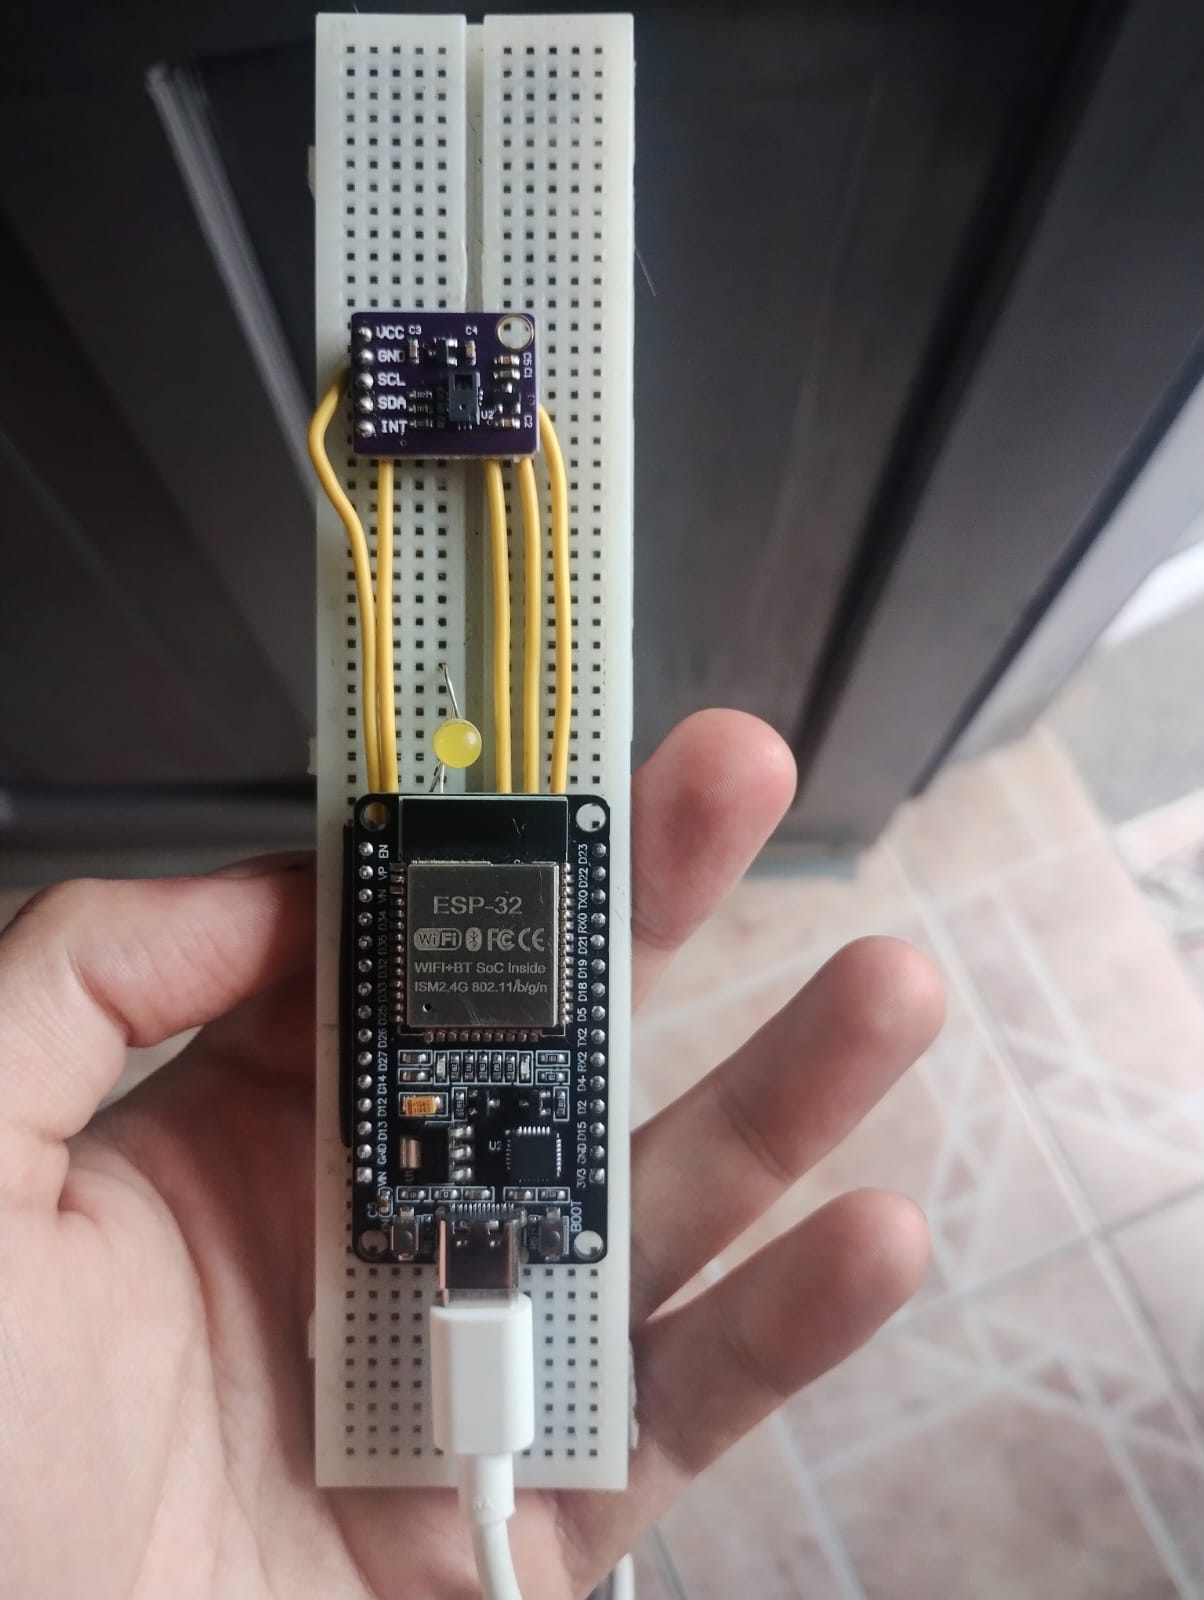
\includegraphics[width=\linewidth]{circuito.jpeg} % \linewidth se ajusta a la columna
      \caption{Vista general del circuito armado}
      \label{fig:circuito}
    \end{figure}

  \subsection{Conexiones y pines}
  Las conexiones se realizaron con alambres de cobre calibre 18, ajustados a la distancia necesaria entre cada pin y acomodados por debajo de la ESP32, con la finalidad de reducir los cables sueltos que  pudieran interferir con los gestos del usuario. Como puede apreciarse en la figura \ref{fig:circuito-debajo}. 
  \begin{itemize}
    \item D15 del ESP32 $\rightarrow$ INT del PAJ7620U2
    \item D26 del ESP32$\rightarrow$ resistencia $220 \Omega \rightarrow$ Anódo (+) del LED
    \item D21 del ESP32$\rightarrow$ SDA del PAJ7620
    \item 3.3V del ESP32 $\rightarrow$ VCC del PAJ7620
    \item GND del ESP32 $\rightarrow$ GND el PAJ7620 $\rightarrow$ Cátodo (-) del LED. 
  \end{itemize}
  
    \begin{figure}[h]
      \centering
      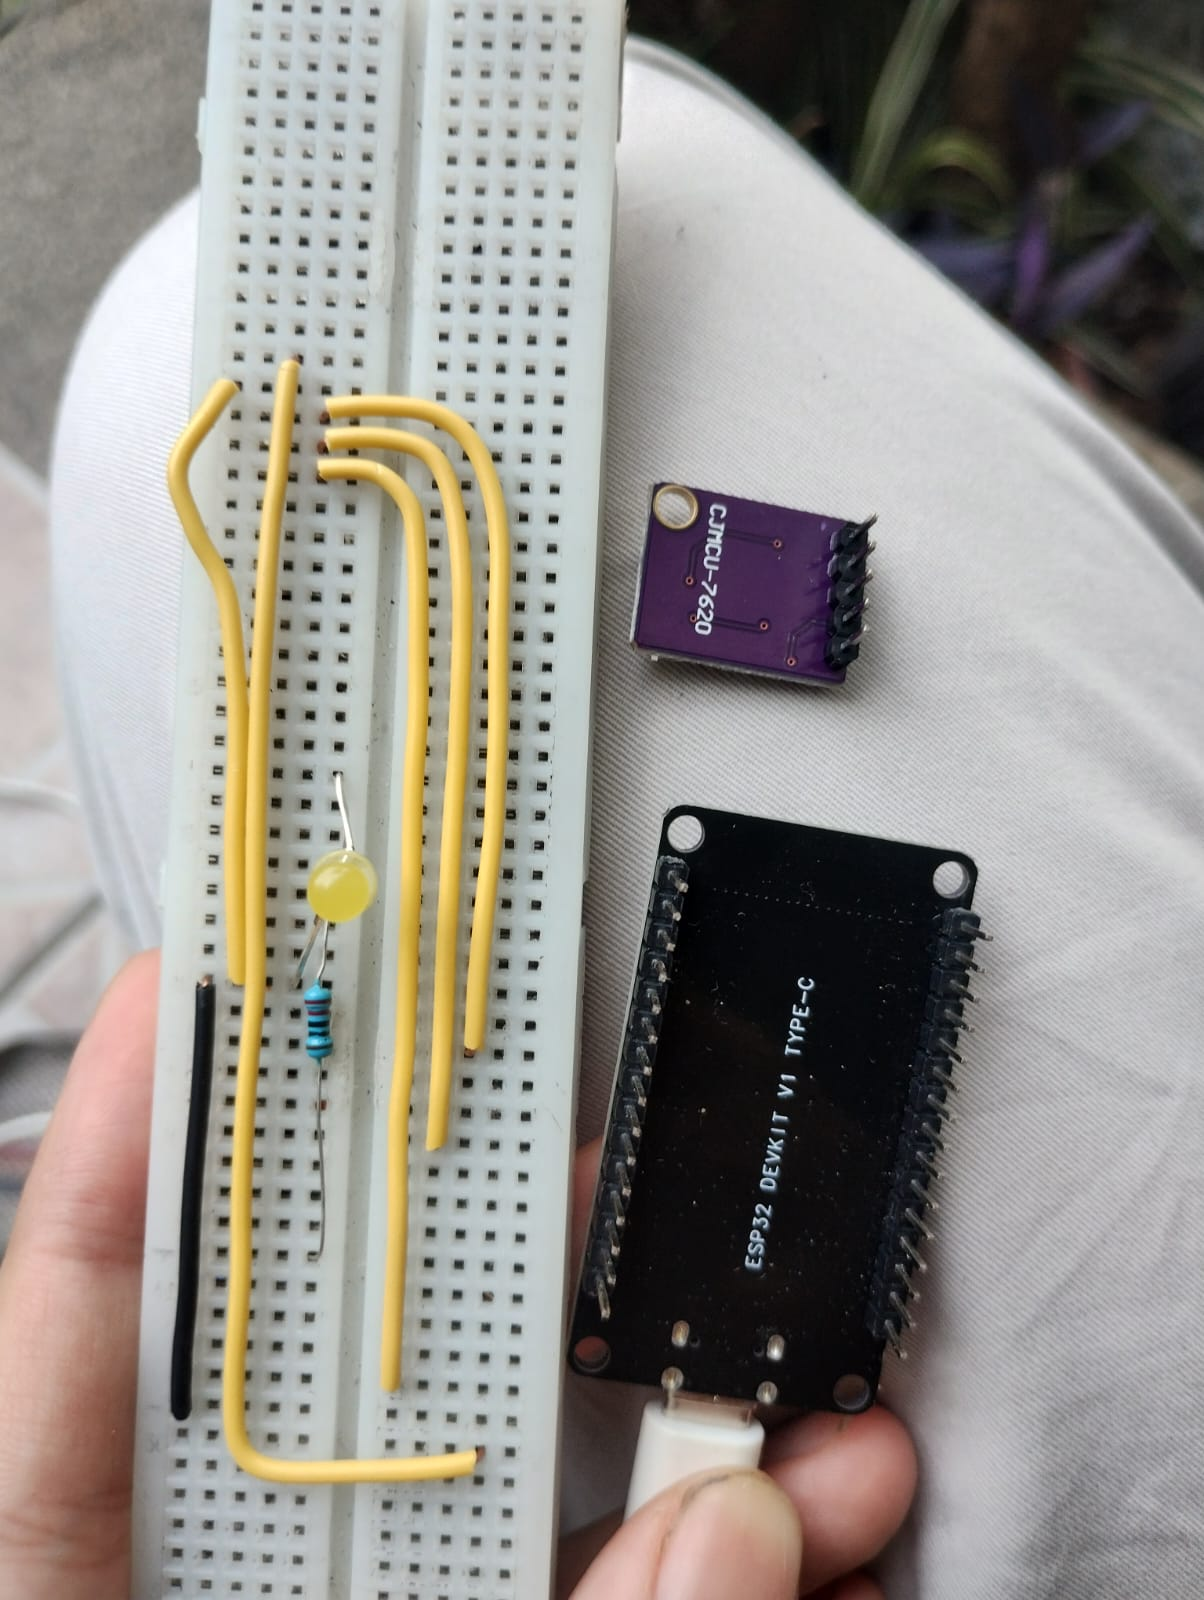
\includegraphics[width=\linewidth]{circuito2.jpeg} % \linewidth se ajusta a la columna
      \caption{Vista el circuito, desde abajo}
      \label{fig:circuito-debajo}
    \end{figure}



\newpage
\section{Conclusiones}

A diferencia de actividades previas, el uso de la librería para el sensor simplificó significativamente el desarrollo de esta Interfaz Hombre-Máquina (HMI). Sus funciones sencillas, directas y de alto nivel facilitaron en gran medida la integración lógica dentro del algoritmo final, delegando el procesamiento complejo al hardware. 

En cuanto al diseño en físico, la eficiencia del protocolo I2C nos permitió optimizar el uso de los cables. Esto nos llevó a organizar las conexiones de la manera más discreta y compacta posible. Además, optar por alambres cortados a la medida en lugar de cables y montar el sistema sobre una protoboard le otorgó la rigidez estructural necesaria para facilitar su manipulación y evitar interferencias o desconexiones físicas durante la interacción del usuario.

Sobre el diseño del algoritmo, el mayor desafío consistió en ajustar con precisión los comandos de detención y selección. Inicialmente, el sobredesplazamiento natural de la mano al intentar detener el cursor generaba señales erroneas, invirtiendo la dirección en vez de frenarla. Para solucionar esto, se implementó una lógica de control inspirada en el comportamiento de un ratón de computadora (clic y doble clic mediante el gesto de ``acercar''). Esta solución no solo eliminó los movimientos indeseados, sino que otorgó mayor fluidez a los desplazamientos durante el cambio de dirección y permitió que las instrucciones del usuario se ejecutaran de forma mucho más definida y controlada.


\section{firma de revisión}
\begin{figure}[h]
    \centering
    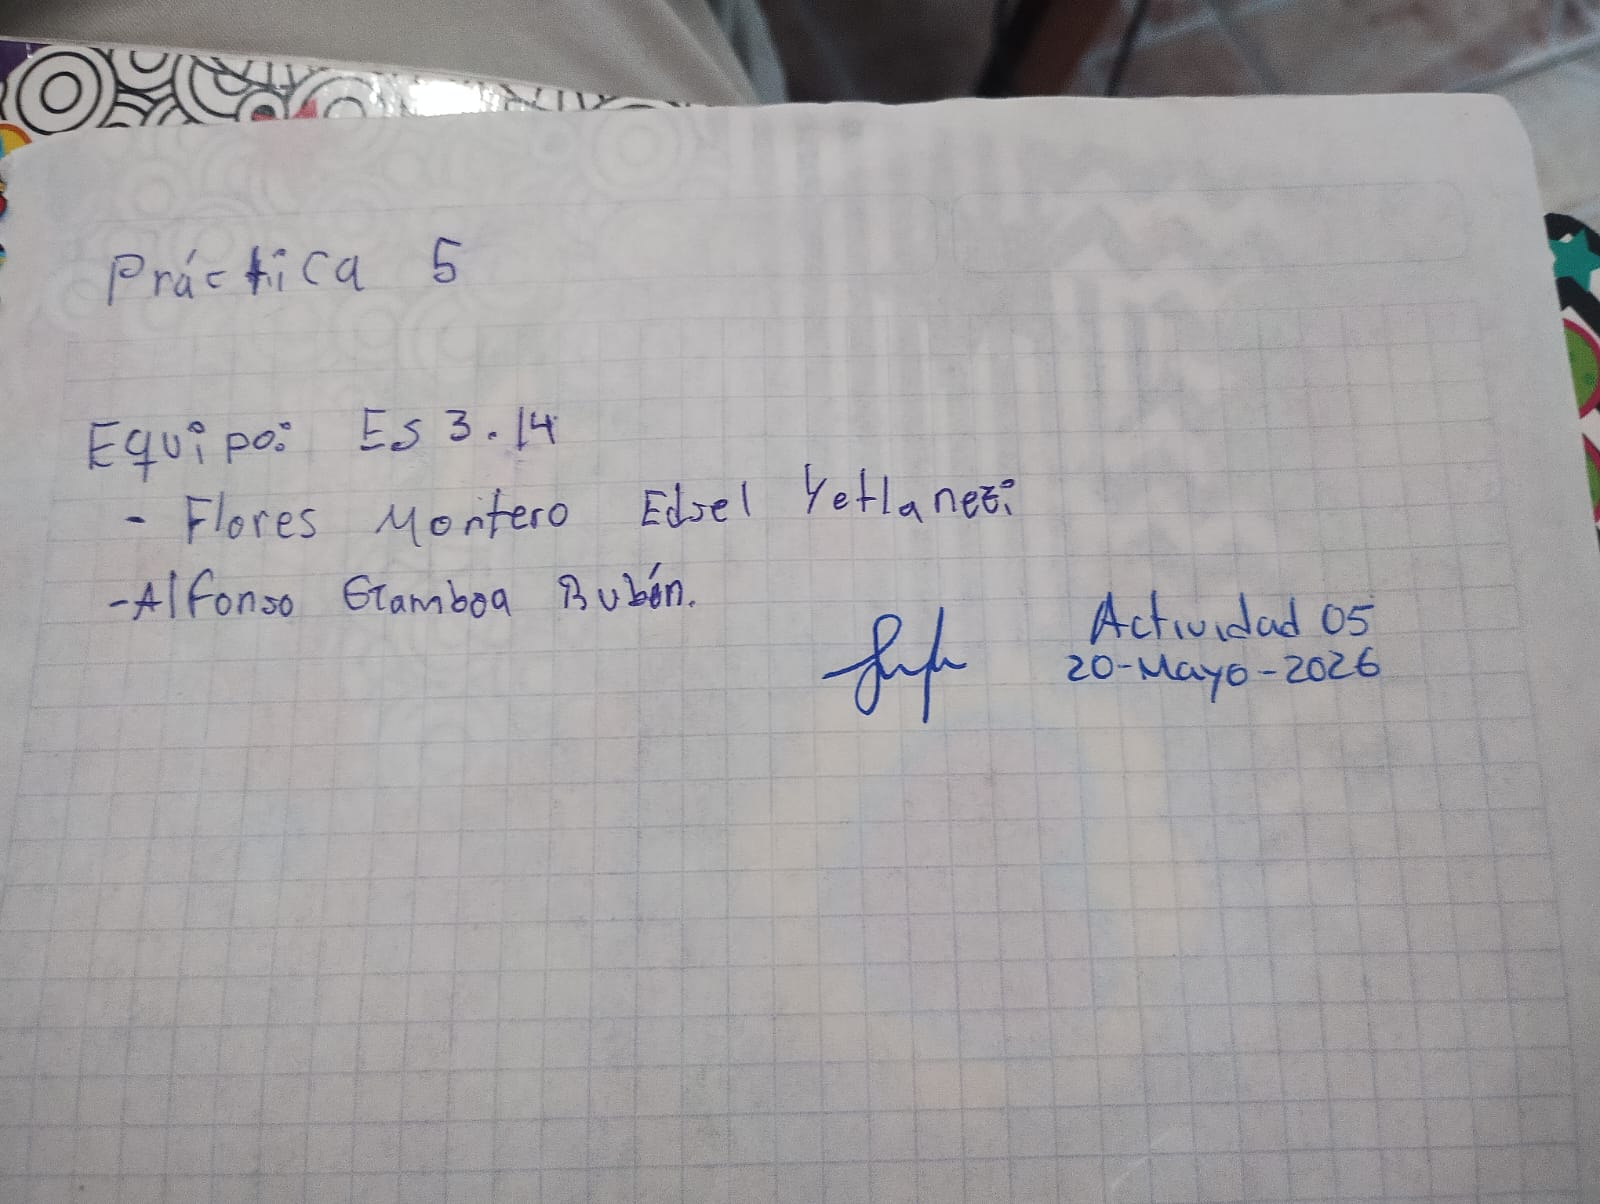
\includegraphics[width=\linewidth]{Firma.jpeg} % \linewidth se ajusta a la columna
    \caption{Firma de revisión}
    \label{fig:Firma}
\end{figure}




% --- REFERENCIAS ---
\printbibliography



\end{document}
